\documentclass[11pt] {article}

%set spacing to 1/2
\usepackage{setspace} 
\onehalfspacing

%load graphics package
\usepackage{graphicx} 


%set continuous line numbering
\usepackage{lineno}
\linenumbers

%Harvard Referencing
\usepackage{natbib}


\title{\textbf{Incorporating isoprene emissions into the P-model for vegetation productivity}
\\[1ex] \large Project Proposal}
\author{Bikem Pastine
\\[1ex] \large bp222@ic.ac.uk}
\date{April 2023}

\begin{document}
    \maketitle

   \section{Supervisors}

    \textbf{Dr. Catherine Morfopoulos}
    \\Reaserch Associate
    \\Department of Life Sciences
    \\Imperial College London
    \\c.morfopoulos@imperial.ac.uk\par

    \vskip 0.2in
    
    \noindent\textbf{Prof. Iain Colin Prentice FRS}
    \\Chair of Biosphere and Climate Impacts and
    \\Director, Leverhulme Centre for Wildfires, Environment and Society
    \\Imperial College London
    \\c.prentice@imperial.ac.uk

    
    \section{Six key words}
    Terrestrial Plants; Net Primary Productivity; P-Model; Earth Observation; Biogenic Volatile Organic Compounds; Heat Dissipation 
    
    \newpage

    \section{Background}

    The P-model is a parameter sparse mechanistic vegetation productivity model. It unifies the Farquhar, von Caemmerer and Berry model for photosynthesis and stomatal conductance with light use efficiency models \citep{P-Modelv1.0}. Underlying the model is the optimality principal stating that plants evolve and adapt to balance between the carbon cost of maintaining transpiration and carboxylation \citep{ZOU2023128855}. Light use efficiency is incorporated in the model by the coordination hypothesis that the maximum rates of carboxylation and electron transport are coordinated to operate close to the interaction light and RuBiSCo limited assimilation rates \citep{P-Modelv1.0}. The P-model successfully models Net Primary Productivity (NPP), explaining 75\% of the variation in NPP gloablly, making it a compelling  model to use to model vegetation productivity.  

    \vskip 0.2in

    \noindent Non-photochemical quenching (NPQ) impacts NPP but is not included explicitly in the P-model.  NPQ protects plants from heat damage. Energy is lost from the photosynthetic pathways as a result of NPQ, negatively impacting the NPP of the plant but protecting it from light induced damage \citep{NPQ_Evolution}. One pathway of heat dissipation is through isoprene emission by plants \citep{morfopoulos_prentice_2014}. Isoprene is the most common Biogenic Volatile Organic Compound. It is emitted instantaneously by plants and has a carbon cost of between 2-20\% of total leaf net carbon assimilation, depending on the ambient temperature. Isoprene also impacts the global energy budget: isoprene emissions are estimated to increase the residence time of methane in the atmosphere by two years and it has complex effects on cloud formation and albedo. Not all plants emit isoprene and its concentrations are highly spatially variable due to a myriad of factors. The short lifetime of isoprene, on the order of 50 minutes to 1.3 days, makes it difficult to measure directly. The oxidation product of isoprene, formaldehyde (HCHO), can be used as a proxy for isoprene at a regional scale as remotely sensed data are readily available.
    
    \section{Proposed Project}
    I plan to incorporate a simplified isoprene emission algorithm in the P-model. The algorithm will be based on the mechanistic isoprene emission model proposed by Dr. Morfopoulos \citep{morfopoulos_prentice_2014}. The algorithm will be incorporated into the python code for the P-model \citep{P-Modelv1.0}. I will run the modified model globally from 2005 to 2020 using the university HPC service. 
   
    \vskip 0.2in
    
    \noindent The modified P-model will be forced with the newly available fAPAR data from the European Space Agency Climate Change Initiative \citep{blessing_2022}. This data improves upon previously available products as it is more coherent and is sensor independent. Using this newly available data to force the P-model will be an improvement on previous studies where the quality and variability in the measurement of fAPAR concerned authors \citep{P-Modelv1.0}, \citep{acclimation_2021}. The remaining data required for the model i.e. air temperature, site elevation, ambient carbon dioxide concentrations etc. has been collated by the research group for previous projects. 

    \vskip 0.2in
    
    \noindent The modelled isoprene emissions will be assessed against satellite observations of isoprene and its proxy, formaldehyde. Atmospheric isoprene is measured using the Cross-tracked Infrared Sounder  since 2020. Beyond this, formaldehyde data are available from Sentinel-5P TROPOMI from 2018 onward and from the Ozone Monitoring Instrument satellite from 2005 onward. Data is open access. Special attention will be given to the inter-annual and seasonal consistency of the modelled isoprene and the observations. 
    

    \section{Budget}
    \begin{itemize}
        \item £60 for printing (due to dyslexia)
        \item £40 for an external hard drive
    \end{itemize}


\newpage

    \section{Timeline}

    \begin{figure}[!ht]
    \centering
    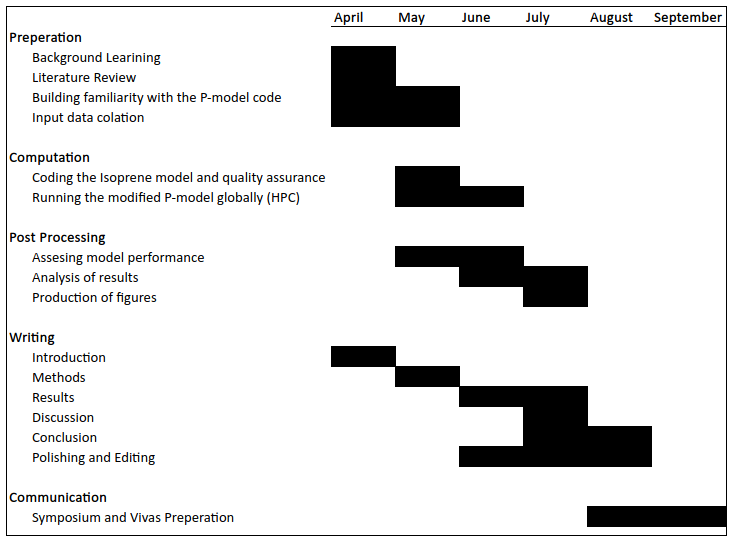
\includegraphics[width=\textwidth]{Timeline.png}
    \caption{Project Gantt Chart}
    \label{timeline}
   \end{figure}
    
    
    
    \newpage
    \bibliographystyle{plain}
    \bibliography{MyBiblio}
    

    
\end{document}